\documentclass[11pt,a4paper,twoside]{article}
\usepackage[top=2cm, bottom=2cm, left=2cm, right=2cm]{geometry}  % nustatomos paraštės
\usepackage[T1]{fontenc}		% LT raidėms su Helvetica
\usepackage[utf8]{inputenc}		% šriftams
%\def\LTfontencoding{L7x}		% LT raidėms su Times New Roman
%\usepackage[L7x]{fontenc}
\usepackage[lithuanian]{babel}	% sulietuvinimas
\usepackage{graphicx}			% paveikslams
\usepackage{caption}			% paveikslu aprašams
\usepackage{subcaption}			% paveikslu aprašams
\usepackage{amsmath}			% formulėms
\usepackage{amsthm}				% sudėtingoms formulėms
\usepackage{amsfonts}			% matematiniams šriftams
\usepackage{pifont}				% šriftams
\usepackage{gensymb}			% matematiniams simboliams
\usepackage{enumerate}			% numeracijai
\usepackage{float}				% paveikslų ir lentelių pozicionavimui
\usepackage[version=3]{mhchem}	% cheminėms formulėms
\usepackage{multirow}			% lentelėms
\usepackage{lmodern}	    	% kitiem šriftam
\usepackage{afterpage}			% formatavimui
\usepackage{setspace}			% tarpui tarp eilučių
\usepackage{hyperref}			% komanda sukuria nuorodas
\hypersetup{					% nuorodos nespalvinamos
	colorlinks,%
	citecolor=black,%
	filecolor=black,%
	linkcolor=black,%
	urlcolor=black
}

\usepackage[scaled]{helvet}			% Helvetica šrifto paketas
\renewcommand{\familydefault}{\sfdefault} % pagrindinio šrifot pakeitimas į Sans, šiuo atveju Helvetica

\begin{document}
\sloppy					% neleidžia tekstui išlįsti į paraštes


\title{$Z^0$ decay into $\mu^{+}$ and $\mu^{-}$}
\author{Nikolajus Elkana Eimutis \\ Taikomoji fizika, Fizikos fakultetas, Vilniaus Universitetas}
\maketitle

\onehalfspace

\paragraph*{Goal:}
Using LHCb open data measure Z boson mass and other important variables (observables?).


\section{Milestones}

\begin{enumerate}
        \item Data is downloaded and ready for local analysis.
        
        \item Theoretical understanding of how LHCb gathers its data is developed.
        
        \item Theoretical understanding of how two muons arise from two protons is developed.

        \item Pratical skill to write root macros is learned.

        \item The data is filtered in such a manner that there is only one evident peak in the Z boson mass graph.

        \item A boson mass graph is drawn, the data is fitted against appropriate theoretical function.
\end{enumerate}
	
% \thispagestyle{empty}			%opcija nenumeruoti pirmojo psl.
\newpage


\section{Theory}
    \begin{enumerate}
        \item Feynman diagrams

        They are figurative depictions of contributions from interactions between particles, which are described by quantum field theory\cite{Jende_Kobel_Pospiech_Bilow_Pedersen_Ould-Saada_Gramstad}.

        \begin{figure}[H]
            \centering

            \subfloat[\centering Muon-antimuon anihilation\cite{Jende_Kobel_Pospiech_Bilow_Pedersen_Ould-Saada_Gramstad}.]{{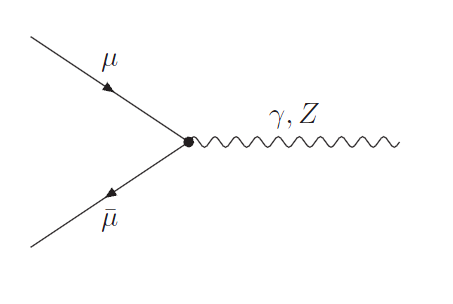
\includegraphics[width=0.5\textwidth]{visuals/002-MuonAntimuonAnihilation.png} }}%
            \subfloat[\centering $Z^0$ decay into muon-antimuon pair\cite{Jende_Kobel_Pospiech_Bilow_Pedersen_Ould-Saada_Gramstad}.]{{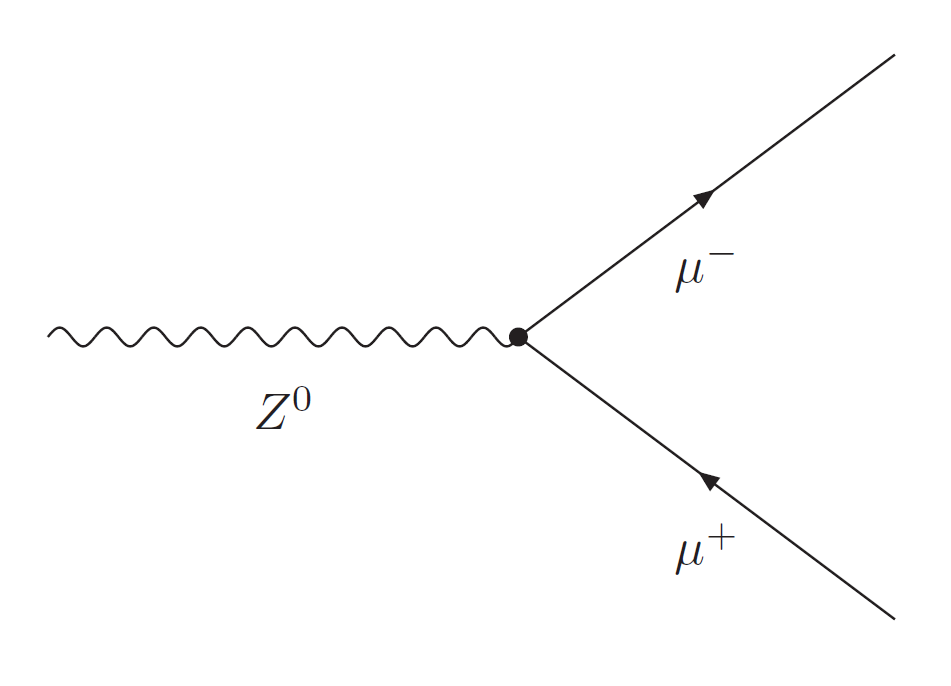
\includegraphics[width=0.5\textwidth]{visuals/001-Z_MyonAntimyon.png} }}%
            
            \caption{Feynman diagrams for the processes with Z boson and muon-antimuon pair.}
            \label{fig:001-Z_MyonAntimyon}
        \end{figure}

        When a quark from one hadron collides with an antiquark of the same flavour form another hadron there is a chance of annihilation. When the net electric charge is zero, they annihilate into virtual photon $\gamma^{*}$ or $Z$ boson\cite{ATLAS_Z_lab}. Due to a short lifetime they soon decay into a pair of leptons. This is so called \textit{Drell-Yan process}.

        \textit{Drell-Yan process} - one of the most important processes that occur in high energy hadron-hadron scattering (for example, proton-proton collisions at LHC). It happens when a quark of one hadron and an antiquark of another hadron annihilate while also creating a virtual photon or $Z$ boson which in turn decays into a pair of oppositely-charged leptons. The energy is almost entirely transformed into mass.

        \begin{figure}[H]
            \centering

            \subfloat[\centering A principal Drell-Yan process diagram\cite{ATLAS_Z_lab}.]{{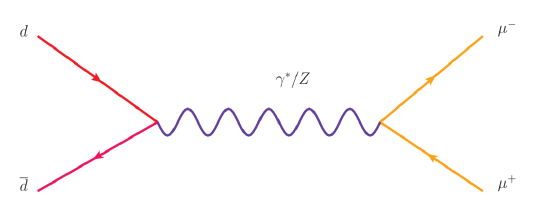
\includegraphics[width=0.5\textwidth]{visuals/003-drell-yan-simple.png} }}%
            \subfloat[\centering A more realistic Drell-Yan process diagram taking into account remnant gluon radiation processes\cite{ATLAS_Z_lab}.]{{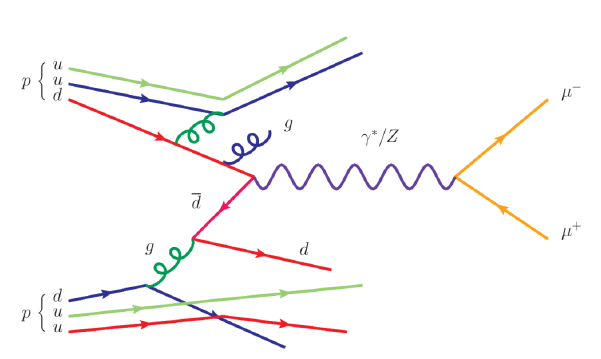
\includegraphics[width=0.5\textwidth]{visuals/004-drell-yan-real.png} }}%
            
            \caption{Feynman diagrams for Drell-Yan processes.}
            \label{fig:002-drell_yan}
        \end{figure}


        \item Processes mimicking $Z$ boson signal

        Due to its short lifetime $Z$ boson is detected by analysing the decay products. Hence, any process producing (in this case) muon-antimuon pair of a mass in the range that we would expect to find the boson would result in a fake signal. It is important to note that the signal can be produced by a bad dimuon candidate, there is no need for a physical process to happen. More on the accuracy and identification efficiency can be found under section 5.


        A few physical processes that produce muons are listed below. Notice that they are of little importance since the produced masses of muons differ vastly from the $Z$ boson decay product. However, single stray muons may induce an error during the $Z$ boson reconstruction stage, if a \textit{Tag and Probe} method was to be used.

        \begin{enumerate}
            \item \textit{pion decay}
            \item \textit{W boson decay}
            \item \textit{Cosmic rays}
        \end{enumerate}


        An important phenomenon to consider when analysing $Z$ boson are "fake signals" coming from virtual photons that have high mass as they are practically indistinguishable from the $Z$ boson.

        
        \item Main graphs drawn when analysing Z boson decay into two muons. What properties are usually analysed?


        These are the parameters analysed in a few different research papers:
        \begin{enumerate}
            \item $G_{\mu}$, $\bar{\alpha}$, $m_Z$ \cite{novikov1999theory};
            \item Muon and Z-boson momentum, pseudorapidity \cite{khodaverdian2019accuracy};
            \item Weinberg angle (indicating the strength of the $W^0$ and $B^0$ bosons mixing), pseudorapidity, tracking and identification efficiencies, $Z$ boson mass cross-section width \cite{ATLAS_Z_lab};
            \item Dimuon invariant mass $m_{\mu^{+} \mu^{-}}$ distribution, transverse momentum $p_T$ distribution, cross section, SPD multiplicity $n_{SPD}$ distribution, tracking efficiency, muon identification efficiency \cite{Bursche:2014ltl}.
        \end{enumerate}
        
        \textbf{[TODO: could add explanations on what each of the parameter means]}

        \textbf{[TODO: could write about why $Z$ boson mass is distribution is fitted againt a convolution of a Gauss or Breit-Wigner distribution]}


        \item Theoretical calculation of Z boson mass from two muons.


        Since $Z$ boson through Drell-Yan process decays into dimuon pair with little energy loss, we could approximate its mass to be that of the \textit{invariant mass} of muon pair.

        \textit{Invariant mass} - a variable that is constant in respect to a moving observer; for a particle with energy $E$ and momentum $\vec{p}$ it is defined as:

        \begin{equation}
            m = \frac{1}{c^2} \sqrt{E^2 - p^2c^2}
            \label{eq:001-invariant-mass}
        \end{equation}

        Invariant mass solves the relativistic problem, where both energy $E$ and momentum $\vec{p}$ measurements change depending on how fast the observer is moving. 

        A more rigorous method for calculating the mass of $Z$ boson could probably be deduced from gauge theory / renormalization / QCD \textbf{[TODO: not sure whether I should add more information on this]}

        Born approximation model, Born process [\textbf{[TODO: ???]}] \cite{khodaverdian2019accuracy}

        

        \item LHCb detector structure, trigger, reconstruction, data validity and error.

        In this section if not explicitly specified, all information is taken (practically word-for-word) from \cite{Bursche:2014ltl} - it contains a very good description about everything.

        \begin{figure}[H]
            \centering

            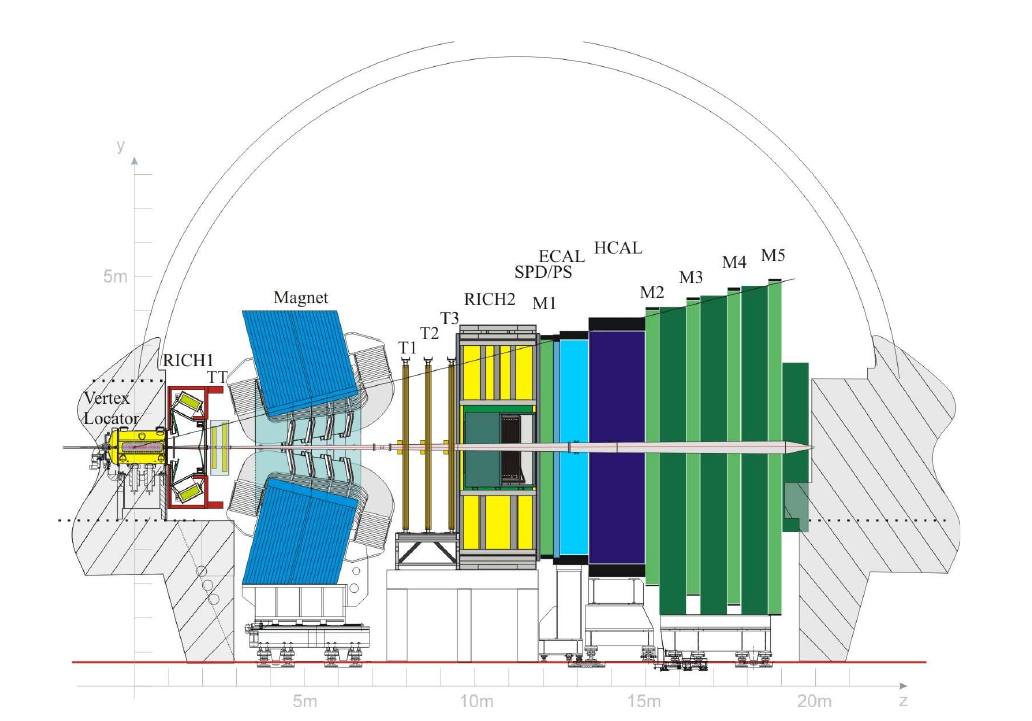
\includegraphics[width=0.7\textwidth]{visuals/005-LHCb-detector.png}
            
            \caption{LHCb detector sketch.}
            \label{fig:001-LHCb_detector}
        \end{figure}

        \begin{figure}[H]
            \centering

            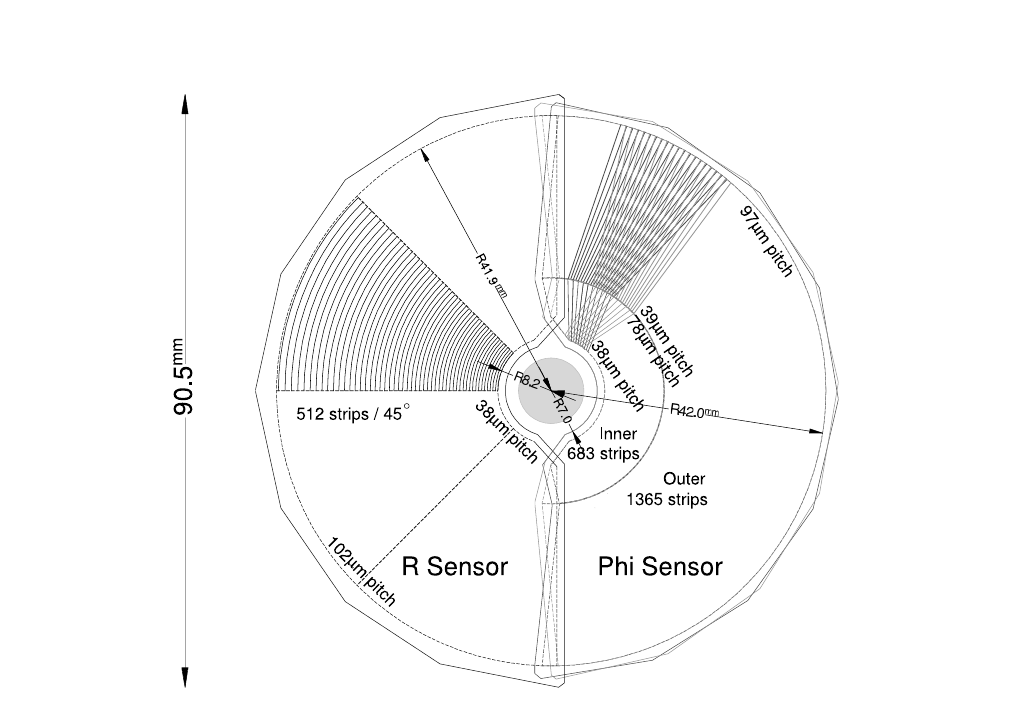
\includegraphics[width=0.7\textwidth]{visuals/006-sensors-in-VeLo.png}
            
            \caption{Sketch of the $r$ and $\phi$ sensors used in VeLo.}
            \label{fig:001-LHCb_detector}
        \end{figure}



        Tracking system consists of:
        \begin{enumerate}
            \item \textbf{Vertex locator (VeLo)} - a silicon strip detector very close to the interaction point measuring the radial and azimuthal coordinates.

            \item \textbf{TT} - another silicon strip detector with two stereo layers at $5^\circ$  in front of a dipole magnet with a peak field strength of $1 T$.

            \item \textbf{T} - another tracking station after the magnet consisting of silicon strip detectors in the forward region (IT) and drift tubes are more central rapidity (OT).
        \end{enumerate}

        Track types:
        \begin{enumerate}
            \item \textbf{VeLo} - tracks that are easured only by the VeLo. Those tracks are mainly used to find \underline{primary vertex and the decay vertices}. The magnetic field integral seen by these tracks is small and this there is \textit{no momentum estimate available}.
            
            \item \textbf{backward} - like VeLo tracks but those tracks are pointing in the backward direction.
            
            \item \textbf{upstream} - VeLo tracks extrapolated to the TT station and \textit{matched to hits in the TT station}. These tracks do see the fringe field of the magnet and this \underline{have a momentum estimate}. These tracks can in principle be reconstructed at very low momentum but practically the momentum acceptance is limited by the search windows in the algorithm to $p_T > 200 MeV$.
            
            \item \textbf{T} - tracks reconstructed in T stations only. These tracks don't see a large magnetic field inside the measured segment but together with the assumption that they originate from the PV \underline{they can get a momentum estimate assigned}. These tracks \underline{play a role as intermediate objects in the reconstruction of other tracks} and also for te understanding of the \underline{contribution of secondary particles to the photons seen in RICH2}. They are also used to \underline{veto charged particles in te neutral hadron reconstruction for jets}.
            
            \item \textbf{downstream} - T tracks matched to hits in the TT station. Those tracks \underline{have measurements on both sides of the dipole magnet and thus a well measured momentum}. For physics analyses they are of special importance for the reconstruction of $K^{0}_{S}$ and $\Lambda$ which often decay after the VeLo.
            
            \item \textbf{long} - tracks that do have measurements both in the VeLo and the T station. Hits in the TT station are not required for a long track and added when found compatible. \underline{If foud these hits improve momentum resolution} and recurse the probability that the long track is a random combination of hits tht does not correspond to a real particle i. e. a ghost. \underline{Long tracks are the major workhorse of the physics analyses}.
            
            \item \textbf{$\mu$ stubs} - tracks reconstructed in the \underline{muon system} only. Their major use is in the \textit{earliest trigger stage}. With the assumption that muons tracks originate from the luminous region \underline{a momentum estimate is possible}. This allows to trigger on \underline{high momentum muons and dimuons}.
            
            \item \textbf{$\mu$ TT} - muon stubs reconstructed offline that are matched to hits in the TT station. Those track are mainly used for the \underline{estimation of the efficiency} for the reconstruction of long tracks.
            
            \item \textbf{TT} - not reconstructed since the TT station has four layers with a stereo angle. Thus a particle leaving hits in all layers would have two points measured that can be reconstructed as a straight line. There is no redundancy in such a easurement and thus no $\chi^2$ and no handle to discriminate ghost tracks.
        \end{enumerate}

        The \textbf{calorimeter} system is mainly designed for the use in the \textbf{trigger} and for \textbf{particle identification}:
        \begin{enumerate}
            \item \textbf{Scintilating pad detector (SPD)} - the first layer. It consists o scintillating pads of different size made from doped polystyrene which are read for each bunch crossing using wavelength shifting fibres. It serves two purposes. In the earliest trigger statge the number of pads that see a signal is used as a \underline{measure of the total occupancy}. Events with less than 10 cells fired are selected by triggers for exclusive processes. The total multiplicity is also used to reject events at the trigger level that require a lot of CPU time in the later software triggers. \textit{Single muon trigger requires the multiplicity to be less than 600 hits and the dimuon trigger asks for less than 900 hits}. The second use of the SPD is \underline{discrimination of electron and photon candidates both at trigger level and offline}. Electrons are more likely to leave a signal in the SPD since that detector doesn't contain absorbers.
            
            \item \textbf{Preshower (PS)} - is built in a similar way as the SPD, but separated from the SPD by a 15 mm lead plate which corresponds to 2.5 electromagnetic radiation lengths. \underline{This is used to discriminate electrons and photons from hadrons}
            
            \item \textbf{Electromagnetic calorimeter (ECAL)} - is a calorimeter build in the shashlik technology. That is a structure of lead tiles interleaved by scintillator tiles which are read out by wavelength shifting fibers. It covers 25 electromagnetic radiation lengths. At very high momentum it saturates which limits the bremsstrahlung correections on electrons and significantly \textit{worsens the mass resolution} in the $Z \rightlongarrow e^{+} e^{-}$.
            
            \item \textbf{Hadronic calorimeter (HCAL)} - is not meant to reconstruct particle candidates to be used in any offline analysis. Its main purpose is to \underline{provide a trigger for full hadronic final states of the beauty hadron}. Therefore compromises have been made - especially in terms of the limited space in the cavern - leading to a calorimeter that uses 5.6 hadronic interaction lengths in only 1.6 meeters.
        \end{enumerate}

        The trigger is organised in three stages:
        \begin{enumerate}
            \item \textbf{L0} - is implemented in hardware and reduces the collision rate from about 20 MHz to 1 MHz.
            \item \textbf{Hlt1} - is executed on standard CPUs.
            \item \textbf{Hlt2} - only logically separated from \textit{Hlt1}. 
        \end{enumerate}



        \begin{figure}[H]
            \centering

            \subfloat[\centering A principal Drell-Yan process diagram\cite{ATLAS_Z_lab}.]{{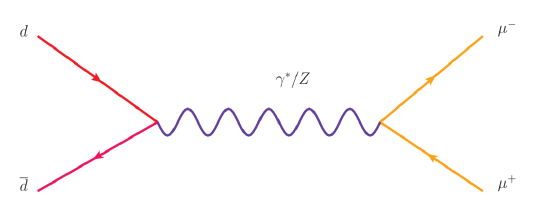
\includegraphics[width=0.5\textwidth]{visuals/003-drell-yan-simple.png} }}%
            \subfloat[\centering A more realistic Drell-Yan process diagram taking into account remnant gluon radiation processes\cite{ATLAS_Z_lab}.]{{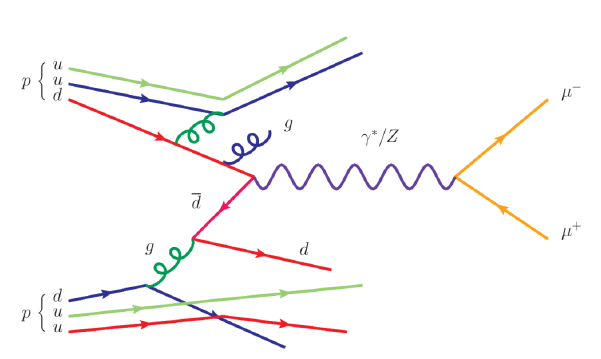
\includegraphics[width=0.5\textwidth]{visuals/004-drell-yan-real.png} }}%
            
            \caption{Feynman diagrams for Drell-Yan processes.}
            \label{fig:001-Z_MyonAntimyon}
        \end{figure}
        
        


        \textit{Tag and probe method} - one well reconstructed and identified muon is combined with a partially reconstructed respectively identified object to a $Z \longrightarrow \mu^{+} \mu^{-}$ candidate.

        [\textbf{[TODO: probably could add more copy pasta]}]

        \item Data types used in LHCb.

        According to official \hyperlink{https://twiki.cern.ch/twiki/bin/view/LHCb/RecommendedTags}{wiki}:

        For real data, new tags mean better description of existing detector. For MC data, the best description is the one used during the simulation step. Therefore, why different Tags for MC?

        \begin{enumerate}
            \item Special settings, Velo open, B field off, ... are identified with a Tag and this Tag needs to be used when reconstructing and analysing the data.
            \item There can be changes in the software which require changes in the databases. Newer software versions might not work anymore with old Tag of database. Requires some intelligence for defining compatible tags.
        \end{enumerate}


        Default tags:
        \begin{enumerate}
            \item \textbf{'DC06'}: “DC06-20081002“ for DDDB and LHCBCONDNote: SIMCOND does not exist for DC06, Simulation flag set to False, bfield polarity = -1 forced
            \item \textbf{'2008'}: “head-20090330” for DDDB, “head-20090402” for LHCBCOND and “sim-20090212” for SIMCOND
            \item \textbf{'MC09'}: “MC09-20090602” for DDDB and “sim-20090402-vc-md100” for SIMCOND, Simulation flag ignored
            \item \textbf{'2009'}: “head-20090617” for DDDB, “head-20090508” for LHCBCOND and “sim-20090508-vc-md100” for SIMCOND. Simulation flag for switching between SIMCOND and LHCBCOND
            \item And some more undocumented tags for each of the year of run (for example "2011", "2012" as used in this analysis).
        \end{enumerate}

        
    \end{enumerate}


\section{Results}
    
\singlespacing
	
	%\phantomsection
	
\bibliographystyle{VUstyle}
\bibliography{mybib}
	
\end{document}
